\documentclass[10pt,a4paper,oneside]{article}
\usepackage[utf8]{inputenc}
\usepackage{draftwatermark} % 设置水印
\SetWatermarkText{DNV Group} % 水印内容
\usepackage{amsmath}
\usepackage{amsfonts}
\usepackage{amssymb}
\usepackage{graphicx}
\usepackage{breqn}
\usepackage{tikz} % system block diagram
\usepackage{textcomp}
\usetikzlibrary{shapes,arrows} % system block diagram
\usepackage{booktabs}
\usepackage[framed,numbered,autolinebreaks,useliterate]{mcode} % matlab code block
\author{Yangang Cao}
\date{February 13, 2019}
\newcommand{\degree}{^\circ}
\tikzset{
	delay/.style    = {draw, thick, rectangle, minimum height = 3em,
		minimum width = 3em},
	sum/.style      = {draw, circle, node distance = 2cm}, 
	prod/.style     = {draw, circle, node distance = 2cm},
	input/.style    = {coordinate}, % Input
	output/.style  = {coordinate} % Output
}
% Defining string as labels of certain blocks.
\newcommand{\product}{$\displaystyle \times$}
\newcommand{\delay}{\large$z^{-1}$}
\begin{document}

\title{First-Order Low/Highpass Filter Design}
\maketitle 

The signal can be seen as a set of partials having different frenquencies and amplitudes. The filter can modify the amplitude of partials according to their frenquency. The two types of filters can be defined according to the following classification:

\begin{itemize}
	\item {\bfseries Lowpass (LP)} filters select low frenquencies up to the cut-off frenquency $f_c$ and attenuate frenquencies higher than $f_c$. Additionally, a resonance may amply frenquencies around $f_c$.
	\item {\bfseries Highpass (HP)} filters select high frenquencies higher than $f_c$ and attenuate frenquencies below $f_c$, possibly with a resonance around $f_c$.
\end{itemize}
The lowpass with resonance is very often used in computer music to simulate an acoustical resonating structure; the highpass filter can remove undesired very low frequencies.\\

A first-order lowpass/highpass filter can be achieved by adding or subtracting (+/--) the output signal from the input signal of a first-order allpass filter.The transfer function of a lowpass/highpass filter is then given by

\[
H(z) = \frac{1}{2}(1 \pm A(z))\quad(LP/HP+/-)
\]
\[
A(z) = \frac{z^{-1} + c}{1 + cz^{-1}}
\]
\[
c = \frac{\tan(\pi f_c/f_S) - 1}{\tan(\pi f_c/f_S) + 1}.
\]

where a tunable first-order allpass $A(z)$ with tuning parameter $c$ is used. The plus sign (+) denotes the lowpass operation and the minus sign (--) the highpass operation. The block diagram in following figure represents the operations involved in performing the low/highpass filtering.
\begin{center}
	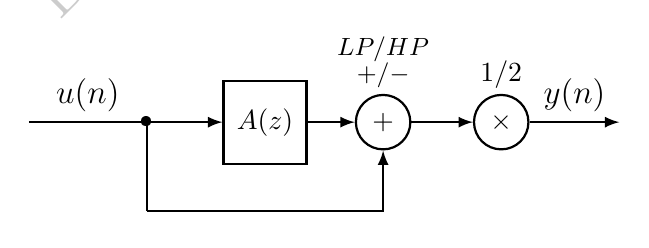
\begin{tikzpicture}[auto, thick, node distance=0.6cm, >=latex, scale = 0.75]
	\draw
	node at (2,0)[delay] (d1) {$A(z)$}
	node at (4,0)[sum] (s1) {$+$} 
	node[above of = s1]{\small$+/-$} node[above of=s1,above=1]{\small{$LP/HP$}}
	node at (6,0) [prod] (p1) {\product} node[above of = p1]{$1/2$};
	
	\draw[-](-2,0) -- node {\large$u(n)$}(0,0);
	\draw[->](0,0) -- node {} (d1);
	\draw[->](d1) -- node {} (s1);
	\draw[->](s1) -- node {} (p1);
	\draw[->](p1) -- node {\large$y(n)$} (8,0);
	\draw[-](0,0) -- node {} (0,-1.5);
	\draw[->](0,-1.5) -| node {} (s1);
	
	\draw
	node at (0,0) {\textbullet};
	
	\end{tikzpicture}
\end{center}

The difference equations of first-order lowpass filter are
\[
x(n) = u(n) - cx(n-1)
\]
\[
y(n) = \frac{1+c}{2}x(n) + \frac{1+c}{2}x(n-1),
\]
and corresponding state and output equations are
\[
x(n) = -cx(n-1) +u(n)
\]
\[
y(n) = \frac{1-c^2}{2}x(n-1) + \frac{1+c}{2}u(n).
\]
A first-order lowpass filter implementation can be obtained by the following {\bfseries Matlab} code.
\begin{lstlisting}
function y = aplowpassunit(audio, para)
% Applies a lowpass filter to the input signal.
% para is the normalized cut-off frequency in (0,1)
c = (tan(pi*para/2)-1) / (tan(pi*para/2)+1);
x = 0;
x_1 = 0;
for n = 1:length(audio)
	x_1 = -c * x + audio(n);
	y(n) = ((1-c^2)/2) * x + (1+c)/2 * audio(n);
	x = x_1;   
end
\end{lstlisting}

The difference equations of first-order highpass filter are
\[
x(n) = u(n) - cx(n-1)
\]
\[
y(n) = \frac{1-c}{2}x(n) + \frac{c-1}{2}x(n-1),
\]
and corresponding state and output equations are
\[
x(n) = -cx(n-1) + u(n)
\]
\[
y(n) = \frac{c^2-1}{2}x(n-1) + \frac{1-c}{2}u(n).
\]
A first-order highpass filter implementation can be obtained by the following {\bfseries Matlab} code.
\begin{lstlisting}
function y = aphighpassunit(audio, para)
% Applies a highpass filter to the input signal.
% para is the normalized cut-off frequency in (0,1)
c = (tan(pi*para/2)-1) / (tan(pi*para/2)+1);
x = 0;
x_1 = 0;
for n = 1:length(audio)
	x_1 = -c * x + audio(n);
	y(n) = ((c^2-1)/2) * x + (1-c)/2 * audio(n);
	x = x_1;  
end
\end{lstlisting}
\end{document}
